\section{Utility and Risk Awearness}
\label{sec:utilityAnRisk}

Classical HTN planners have several advantages over classical planners, but they lack any concept of utility. Classical HTN planners are satisfied when a solution is found, but in the real world, this is rarely sufficient. In the real world, we are typically interested in finding an optimal solution in some sense. For instance, we may only be interested in solutions that are safe, fast, or inexpensive. In this section, we will provide an overview of the notion of utility and how it can be utilized to guide the planning process.

\subsection{Utility}
The core concept of utility revolves around modeling the outcomes of an action or situation based on a set of criteria or metrics, which allows us to rank actions or outcomes and choose the most preferable option. Mathematically, utility can be represented via a set of binary relations over a set of actions or situations $\mathbf{\Sigma}$ \cite{fishburn1968utility}.

\begin{Tdef}[Preference-indifference relation $\preceq$]
    The preference-indifference relation $\preceq$ is a binary relation over a set of actions/situations $\mathbf{\Sigma}$ that satisfies the following:
    $$\forall \sigma_1, \sigma_2 \in \Sigma : \sigma_1 \preceq \sigma_2 \vee \sigma_1 \npreceq \sigma_2$$
    $\sigma_1 \preceq \sigma_2$ means that $\sigma_1$ is not preferred to $\sigma_2$.
\end{Tdef}

\begin{Tdef}[Strict preference relation $\prec$]
    The strict preference relation $\prec$ is a binary relation over a set of actions/situations $\mathbf{\Sigma}$ that satisfies the following:
    $$\forall \sigma_1, \sigma_2 \in \Sigma : \sigma_1 \prec \sigma_2 \Longleftrightarrow \sigma_1 \preceq \sigma_2 \wedge \sigma_2 \npreceq \sigma_1$$
    $\sigma_1 \prec \sigma_2$ means that $\sigma_2$ is preferred to $\sigma_1$.
\end{Tdef}


\begin{Tdef}[Indifference relation $\sim$]
    The indifference relation $\sim$ is a binary relation over a set of actions/situations $\mathbf{\Sigma}$ that satisfies the following:
    $$\forall \sigma_1, \sigma_2 \in \Sigma : \sigma_1 \sim \sigma_2 \Longleftrightarrow \sigma_1 \preceq \sigma_2 \wedge \sigma_2 \preceq \sigma_1$$
    $\sigma_1 \sim \sigma_2$ means that $\sigma_1$ is indifferent to $\sigma_2$.
\end{Tdef}

The previous binary relations form an invaluable framework that enables us to rank solutions given that we have a model that can map any action/situation to a numeric value (utility). It is essential to recognize that utility and value do not constitute the same concept. For example, in the context of commuting to work, one can use the train or a taxi. The train would cost two dollars, whereas the taxi would cost twenty. These values do not take into consideration factors such as comfort, speed, or emissions. Concrete values such as cost and time are objective, whereas utility is quite subjective. An agent with an emphasis on comfort would give the train a lower utility score, while an agent with an emphasis on reducing emissions would give the train a higher utility score.


\subsection{Utility based HTN planning}
One way of utilizing utility to guide an HTN planner is to assign each operator a utility score, but this is insufficient. HTN structures are intrinsically hierarchical, and the utility of a task is not necessarily identical to the utility of its subtasks. A significantly better approach is to assign a utility score to each operator, method, and compound task. The utility of a task is then the sum of its own utility and the utility of its most preferred subtask. It is essential to bear in mind that utility is extremely dynamic, and thus the planner needs to be able to recalculate the utility of each task as the planning process progresses or whenever the state of the environment changes.

\begin{figure}[H]
    \centering
    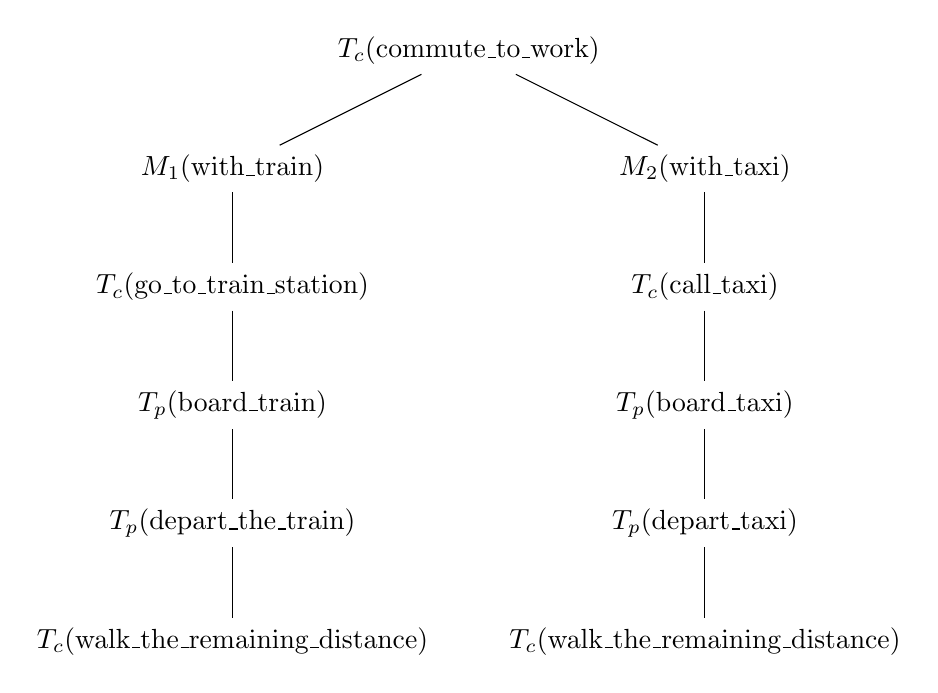
\begin{tikzpicture}
        \node {$T_c$(commute\_to\_work)} [sibling distance = 6cm]
            child { 
                node{$M_1$(with\_train)} 
                child{ 
                        node{$T_c$(go\_to\_train\_station)}
                        child {
                            node{$T_p$(board\_train)}
                            child {
                                node{$T_p$(depart\_the\_train)}
                                child{
                                    node{$T_c$(walk\_the\_remaining\_distance)}
                                }
                            }
                        }
                    }
                }
            child {
                node{$M_2$(with\_taxi)}
                child{ 
                        node{$T_c$(call\_taxi)}
                        child {
                            node{$T_p$(board\_taxi)}
                            child {
                                node{$T_p$(depart\_taxi)}
                                child{
                                    node{$T_c$(walk\_the\_remaining\_distance)}
                                }
                            }
                        }
                    }
                };
    \end{tikzpicture}
    \caption{A simple HTN task network for commuting to work.}
    \label{fig:commute_to_work}
\end{figure}
Figure ~\ref{fig:commute_to_work} shows a simple HTN task network for commuting to work. This example will help us to illustrate the necessity of having a utility score for each HTN construct. If we exclusively assign utility values to the operators, there will be no way to express whether an agent prefers or dislikes using the train for example. The compound task \qq{walk\_the\_remaining\_distance} can be reached via two distinct paths, and it would be illogical to assign it the same utility in both scenarios. The compound task \qq{commute\_to\_work} itself could have an inherently low utility value if the agent prefers to work from home.

We will refrain from providing a concrete algorithm for integrating utility into HTN planning since it is highly dependent on the search strategies implemented by the planner and because it has already been done in \cite{alnazer2019htn} \cite{georgievski2014utility} \cite{alnazer2022risk}. However, we will go over our own implementation in detail later on.

\subsection{Expected utility}
Basic utility is an effective tool for comparing solutions and ensuring that the agent always chooses the solution with the most preferable outcome. However, basic utility assumes that the world is deterministic and each action has only one outcome, which has a significant impact on its applicability in the real world, where uncertainty is a fundamental challenge.
To illustrate the limitations of basic utility, consider the following scenario shown in Figure~\ref{fig:expected_utility} in which an agent is offered the choice between two actions, $\sigma_1$ and $\sigma_2$. There are two possible outcomes for action $\sigma_1$: the agent will receive three dollars 40\% of the time, and nothing the remaining 60\% of the time. Action $\sigma_2$ also has also two possible outcomes: 10\% of the time, the agent will receive seven dollars, and 90\% of the time, it will receive nothing.

\begin{figure}[H]
    \centering
    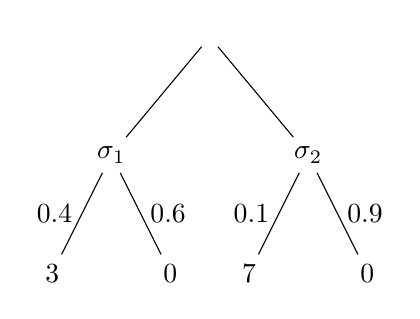
\begin{tikzpicture}
        \node {} [sibling distance = 2.5cm]
            child{
                node{$\sigma_1$}[sibling distance = 1.5cm]
                child{node{3} edge from parent node [left] {0.4}}
                child{node{0} edge from parent node [right] {0.6}}
            }
            child{
                node{$\sigma_2$}[sibling distance = 1.5cm]
                child{node{7} edge from parent node [left] {0.1}}
                child{node{0} edge from parent node [right] {0.9}}
            };
        \end{tikzpicture}
        \caption{A simple example of expected utility.}
        \label{fig:expected_utility}
\end{figure}

If the agent is acting solely on the basis of basic utility, it will always choose action $\sigma_2$, since its utility value is greater, whereas a rational agent will virtually always choose action $\sigma_1$ because it has a greater expected utility:
$$ E(\sigma_2) = 0.1 \times 7 + 0.9 \times 0  \prec E(\sigma_1) = 0.4 \times 3 + 0.6 \times 0 $$

